\documentclass[a4paper,norsk, 10pt]{article}
\usepackage[utf8]{inputenc}
\usepackage{verbatim}
\usepackage{listings}
\usepackage{graphicx}
\usepackage[english]{babel}
\usepackage{a4wide}
\usepackage{color}
\usepackage{amsmath}
\usepackage{float}
\usepackage{amssymb}
\usepackage[dvips]{epsfig}
\usepackage[toc,page]{appendix}
\usepackage[T1]{fontenc}
\usepackage{cite} % [2,3,4] --> [2--4]
\usepackage{shadow}
\usepackage{hyperref}
\usepackage{titling}
\usepackage{marvosym }
\usepackage{subcaption}
\usepackage[noabbrev]{cleveref}
\usepackage{cite}
\usepackage{todonotes}


\setlength{\droptitle}{-10em}   % This is your set screw

\setcounter{tocdepth}{2}

\lstset{language=c++}
\lstset{alsolanguage=[90]Fortran}
\lstset{alsolanguage=Python}
\lstset{basicstyle=\small}
\lstset{backgroundcolor=\color{white}}
\lstset{frame=single}
\lstset{stringstyle=\ttfamily}
\lstset{keywordstyle=\color{red}\bfseries}
\lstset{commentstyle=\itshape\color{blue}}
\lstset{showspaces=false}
\lstset{showstringspaces=false}
\lstset{showtabs=false}
\lstset{breaklines}
\title{STK4900 Oblig1}
\author{Daniel Heinesen, daniehei}
\begin{document}
\maketitle


\section*{Exercise 1}


\section*{Exercise 2}
\subsection*{a)}

The data we are looking at is the systolic blood pressure for $36$ people divided into three groups determined by their age. These groups are $30-45$ years, $46-59$ years and $60-75$ years. 

\begin{table}[!htbp] \centering 

\begin{tabular}{@{\extracolsep{5pt}}lccccccc}  
\\[-1.8ex]\hline 
\hline \\[-1.8ex] 
Age Group & \multicolumn{1}{c}{N} & \multicolumn{1}{c}{Mean} & \multicolumn{1}{c}{St. Dev.} & \multicolumn{1}{c}{Min} & \multicolumn{1}{c}{Pctl(25)} & \multicolumn{1}{c}{Pctl(75)} & \multicolumn{1}{c}{Max} \\ 
\hline \\[-1.8ex] 
All & 36 & 138.806 & 25.749 & 104 & 117.5 & 156.2 & 214 \\ 
$30-45$ years & 12 & 122.167 & 15.338 & 104 & 112 & 129 & 160 \\
$46-59$ years & 12 & 139.083 & 22.625 & 108 & 121.5 & 157.8 & 174 \\ 
$60-75$ years & 12 & 155.167 & 27.719 & 110 & 138 & 164 & 214 \\
\hline \\[-1.8ex] 
\end{tabular} 
\caption{A table showing different measures for the distribution of the systolic blood pressure for the three age groups, and the entire group as a whole. The increase in all the measures for the higher age groups seems to indicate a correlation between age and blood pressure.}   \label{tab:blood_summary} 

\end{table} 


If we look at table \ref{tab:blood_summary} we see the numerical summary of the blood pressure of the three age groups, and the group as a whole. From the mean column, we see that mean blood pressure seems to increase with increasing age group. This is also the case for all the other measures see in the table. This seems to indicate that there is some relationship between systolic blood pressure and age. \todo{This may be just repetition of the caption...}


\begin{figure}[!htbp]
\centering
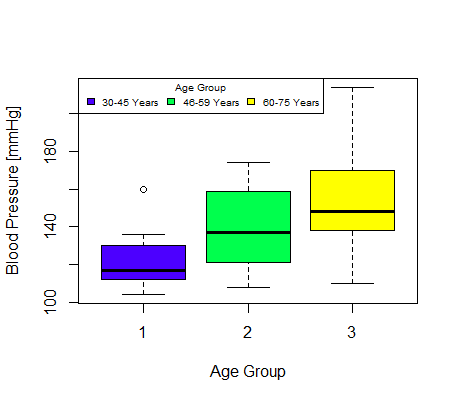
\includegraphics[scale=0.8]{blood_box.png}
\caption{Boxplots showing the distribution of the blood pressure of the three age groups.}\label{fig:blood_box}
\end{figure}


From fig. \ref{fig:blood_box} we see that there is a clear increase in blood pressure with age. Both the median, max and min increases with age. This is exactly what we saw in tab. \ref{tab:blood_summary} -- a difference is that in the table the mean was given, while in the box plot the median is given --. What we can see clearer from the plot is that the distributions also become wider as age increase. The interquartile width of the middle age group is quite wide, and overlaps with the other groups. This can make this group a bit more difficult to get a significant result from.

All in all, both the numerical summary, tab. \ref{tab:blood_summary}, and the box plot, fig. \ref{fig:blood_box}, seems to show the same: A increase in systolic blood pressure as age increases.

\subsection*{b)}

We now want to look close at whether blood pressure varies between the different age groups. Above we used qualitative reasoning to to argue that this is the case. Now we want a quantified measure of this. To do this we will use a one-way ANOVA. 

For the ANOVA we have the following hypotheses:
\begin{itemize}
  \item $H_0: \mu_1 = \mu_2 = \mu_2$
  \item $H_a:  \mu_1 \neq \mu_2 \neq \mu_2$
\end{itemize}

In word: We have a null hypothesis that the mean blood pressure of all the groups are the same, and an alternative hypothesis that this is not that case. For the ANOVA to be valid, we need to assume that: 

\begin{itemize}
  \item The observations are independent of one another
  \item The observations in one group are a random sample with a normal distribution $N(\mu_k,\sigma^2)$
\end{itemize} 



% latex table generated in R 3.5.2 by xtable 1.8-3 package
% Thu Mar 07 14:02:58 2019
\begin{table}[!htbp]
\centering
\begin{tabular}{lrrrrr}
  \hline
 & Df & Sum Sq & Mean Sq & F value & Pr($>$F) \\ 
  \hline
Age Group & 2 & 6535.39 & 3267.69 & 6.47 & 0.0043 \\ 
  Residuals & 33 & 16670.25 & 505.16 &  &  \\ 
   \hline
\end{tabular}
\caption{A table showing the result of an ANOVA test on the blood pressure dataset. We see that we have a high F-value, leading to a small, significant p-value.}\label{tab:blood_anova}

\end{table}


From tab. \ref{tab:blood_anova} we see that we get a small p-value of $p=0.0043$. This is below the $p=0.05$ mark which is standard to use as the limit of significance. This means that we can throw out that null hypothesis, and conclude that blood pressure indeed varies across the age groups \footnote{It is normally bad practice to interpret the p-value in an article, but since this is an oblig, it is done here.}


\subsection*{c)}

We are now going to try to use a categorical regression on the data set. We are going to use treatment-contrast with group 1, the youngest, as the reference group. This means that our model will look like

\begin{equation}
y_i = \mu_1 + (\mu_2-\mu_1)\cdot x_{1,i} + (\mu_2-\mu_1)\cdot x_{2,i} + \epsilon_i,
\end{equation}

where $\epsilon_i$ is a normally distributed error term, $\mu_j$ is the mean of the different age groups, and

\begin{equation}
x_{j-1,i} = 
\begin{cases}
1 \text{	for $i$ in group $j$} \\
0 \text{	else}
\end{cases}.
\end{equation}
This means that if patient is in group 2, then $x_{1,i} = 1$ and $x_{2,i} = 0$, and vis versa if the patient is in group 3. If the patient is in group 1, both will be $0$.

% latex table generated in R 3.5.2 by xtable 1.8-3 package
% Thu Mar 07 15:06:19 2019
\begin{table}[!htbp]
\centering
\begin{tabular}{rrrrr}
  \hline
 & Estimate & Std. Error & t value & Pr($>$ $|$t$|$) \\ 
  \hline
(Intercept) & 122.1667 & 6.4882 & 18.83 & 0.0000 \\ 
  Age Group 2 & 16.9167 & 9.1757 & 1.84 & 0.0742 \\ 
  Age Group 3 & 33.0000 & 9.1757 & 3.60 & 0.0010 \\ 
  \hline
   \multicolumn{5}{l}{Residual standard error: 22.48 on 33 degrees of freedom} \\
	\multicolumn{5}{l}{Multiple R-squared:  0.2816,	Adjusted R-squared:  0.2381} \\
	\multicolumn{5}{l}{F-statistic: 6.469 on 2 and 33 DF,  p-value: 0.004263} \\
   \hline
\end{tabular}
\caption{The summary of the categorical regression of the blood pressure with respect to the age groups.}\label{tab:blood_reg}
\end{table}

In tab. \ref{tab:blood_reg} we see the summary of the regression model with the age groups as a categorical predictor variable. The intercept in the table is the mean of the youngest age group $\mu_1 = 122.167$ --  our reference group --. The slopes of the two variables can be interpreted as how much the mean of blood pressure increases if you are in that age group, compared to the reference group. E.g. if you are in age group 2, we will expect your blood pressure to be $33.0$ mmHg higher than the mean of the youngest group, i.e. it is expected to be $155.167$ mmHg.

We can look at the p-values of tab. \ref{tab:blood_reg} we see that the p-value for age group 3 is $p=0.001$. This means that the increase of $33$ mmHg is significant. But for group 2 the p-value is just $0.0742$, which means that this increase is not significant, so we can not say that we have an $17$ mmHg increase compared  with the reference. This might have to do with what we see in the box plots \ref{fig:blood_box}, where the distribution of the second age group is very wide. The reason might also be due to a non linear dependence on age.

We also see that we have a low $R^2 = 0.2816$, which means that the blood pressure is not fully described by the age groups.

But all in all we see that the we have a good regression model for group 1 and 3, with the change in group 2 not being significant. So there is some significant variation between the age groups, as we saw with the ANOVA. \todo{Look over and rewrte...}

\end{document}

